\documentclass{beamer}

\usepackage{mathtools}
\usepackage{tikz}
\usepackage{pgfplots}
\usetikzlibrary{calc,positioning,arrows,decorations.markings}
\pgfplotsset{compat=1.14}

% --------------------------------------------------------- continue number counter over multiple slides
\usepackage{enumitem}
\setenumerate[1]{label=\arabic*.}

\setitemize{label=\usebeamerfont*{itemize item}%
  \usebeamercolor[fg]{itemize item}
  \usebeamertemplate{itemize item}}

\newcounter{ResumeEnumerate}

% --------------------------------------------------------- x'ed out arrow
\newcommand*{\StrikeThruDistance}{0.2cm}%
\newcommand*{\StrikeThru}{\StrikeThruDistance,\StrikeThruDistance}%
\tikzset{
  strike thru arrow/.style={
    decoration={
      markings, mark=at position 0.5 with {
        \draw [red, very thick, solid,-] ++ (-\StrikeThruDistance,-\StrikeThruDistance) -- ( \StrikeThruDistance, \StrikeThruDistance);
        \draw [red, very thick, solid,-] ++ (-\StrikeThruDistance,\StrikeThruDistance) -- (\StrikeThruDistance, -\StrikeThruDistance);
      }
    },
    postaction={decorate},
  }
}

% --------------------------------------------------------- abbrev
\newcommand{\goedel}[1]{\langle #1 \rangle}
\newcommand{\nats}{\mathbb{N}}
\newcommand{\reals}{\mathbb{R}}
\newcommand{\ints}{\mathbb{Z}}

\newcommand{\setup}{\textbf{SETUP} }
\newcommand{\asign}{\textbf{ASIGN} }
\newcommand{\averify}{\textbf{AVERIFY} }
\newcommand{\verify}{\textbf{VERIFY} }
\newcommand{\keygen}{\textbf{KGEN}}

\newcommand{\mespace}{\mathcal{M}}
\newcommand{\sspace}{\mathcal{S}}
\newcommand{\uspace}{\mathcal{U}}
\newcommand{\kspace}{\mathcal{K}}
\newcommand{\kfspace}{\mathcal{F}}


% --------------------------------------------------------- beamer/document setup
\mode<presentation>

\title{Concurrent Signatures}
% \subtitle{subtitle}

\author{Samir Benzammour}
\date{24th March 2020}
 
\institute[RWTH]{
  Algorithms and Computational Complexity\\
  RWTH Aachen University
}

% fonts etc
\usetheme{Madrid}
\usecolortheme{default}
\usefonttheme{professionalfonts}

\AtBeginSection[]
{
  \begin{frame}
    \frametitle{Outline}
    \tableofcontents[currentsection]
  \end{frame}
}

\AtBeginSubsection[]
{
  \begin{frame}
    \frametitle{Outline}
    \tableofcontents[currentsubsection]
  \end{frame}
}


\begin{document}


\frame{\titlepage}

% --------------------------------------------------------- Global
\begin{frame}
	\frametitle{Outline}
	\tableofcontents
\end{frame}

% --------------------------------------------------------- Introduction
\section{Introduction}
\begin{frame}
	\frametitle{Concurrent Signature Protocol}

	\begin{itemize}
		\item Describing signature exchange between A(lice) and B(ob)
		\item Initial signer has to generate keystone
		\item Matching signer responds by using the same keystone-fix
		\item Alice and Bob both run \setup to set public variables
			\begin{itemize}
				\item A's and B's public- and private keys are $X_A$, $x_a$ and $X_B$, $x_B$, respectively
			\end{itemize}
	\end{itemize}
\end{frame}

\begin{frame}
	\frametitle{Concurrent Signature Protocol}

	\begin{enumerate}
		\item A picks a random keystone $k\in\kspace$ and computes $f = \textbf{KGEN}(k)$
		\item A computes ambiguous signature with $M_A \in \mespace$ being A's message 
			$$\sigma_A \coloneqq \goedel{s_A,h_A,h} = \asign(X_A, X_B, x_A, f, M_A)$$ 
		\item B verifies signature by checking
			$$\averify(\goedel{s_A, h_A, f}, X_A, X_B, M_A) = accept$$
			reject otherwise
		\setcounter{ResumeEnumerate}{\value{enumi}}
	\end{enumerate}
\end{frame}


\begin{frame}
	\frametitle{Concurrent Signature Protocol}

	\begin{enumerate}[start=\numexpr\value{ResumeEnumerate}+1]
		\item B picks message $M_B \in \mespace$ and creates own ambiguous signature
		$$\sigma_B \coloneqq \goedel{s_B,h_B,h} = \asign(X_B, X_B, x_A, f, M_B)$$
		\item A verifies this time with
			$$\averify(\goedel{s_B, h_B, f}, X_B, X_A, M_B) = accept$$
			with $f$ same keystone fix as before
		\item A sends keystone to B
	\end{enumerate}
\end{frame}

\subsection{Fair Signature Exchange}
% Fair Signature Exchange (Example)
\begin{frame}
	\frametitle{Fair Signature Exchange (Example)}

	\begin{itemize}
		\setlength\itemsep{1em}
		\item<1-> Two parties Alice and Bob
		\item<2-> Want to sign an item (e.g. a contract)\vspace*{.5cm}
		\item[]<3-> 
			\begin{center}			
				\begin{tikzpicture}[node distance=2cm,auto,>=stealth']
					\node[] (bob) {Bob};
					\node[left = of bob] (alice) {Alice};
					\node[below of=bob, node distance=3cm] (bobground) {};
					\node[below of=alice, node distance=3cm] (aliceground) {};
					
					% vertical lines
					\draw (alice) -- (aliceground);
					\draw (bob) -- (bobground);

					% signs contract -> receives signed contract
					% \draw[->, dashed] ($(alice)!0.2!(aliceground)$) -- node[left, scale=1, pos=-.02]{signs contract} ($(bob)!0.25!(bobground)$);
					% \draw($(bob)!0.25!(bobground)$) -- node[right, scale=1, xshift=0.1cm]{receives signed contract} ($(bob)!0.25!(bobground)$);
				\end{tikzpicture}
			\end{center}
	\end{itemize}
\end{frame}

\begin{frame}
	\frametitle{Fair Signature Exchange (Example)}

	\begin{itemize}
		\setlength\itemsep{1em}
		\item Two parties Alice and Bob
		\item Want to sign an item (e.g. a contract)\vspace*{.5cm}
		\item[]
			\begin{center}			
				\begin{tikzpicture}[node distance=2cm,auto,>=stealth']
					\node[] (bob) {Bob};
					\node[left = of bob] (alice) {Alice};
					\node[below of=bob, node distance=3cm] (bobground) {};
					\node[below of=alice, node distance=3cm] (aliceground) {};
					
					% vertical lines
					\draw (alice) -- (aliceground);
					\draw (bob) -- (bobground);

					% signs contract -> receives signed contract
					\draw[->, dashed] ($(alice)!0.2!(aliceground)$) -- node[above, scale=0.6]{signs contract} ($(bob)!0.25!(bobground)$);
					% \draw($(bob)!0.25!(bobground)$) -- node[right, scale=1, xshift=0.1cm]{receives signed contract} ($(bob)!0.25!(bobground)$);
				\end{tikzpicture}
			\end{center}
	\end{itemize}
\end{frame}

\begin{frame}
	\frametitle{Fair Signature Exchange (Example)}

	\begin{itemize}
		\setlength\itemsep{1em}
		\item Two parties Alice and Bob
		\item Want to sign an item (e.g. a contract)\vspace*{.5cm}
		\item[]
			\begin{center}			
				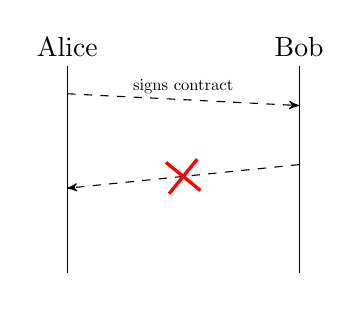
\begin{tikzpicture}[node distance=2cm,auto,>=stealth']
					\node[] (bob) {Bob};
					\node[left = of bob] (alice) {Alice};
					\node[below of=bob, node distance=3cm] (bobground) {};
					\node[below of=alice, node distance=3cm] (aliceground) {};
					
					% vertical lines
					\draw (alice) -- (aliceground);
					\draw (bob) -- (bobground);

					% signs contract -> receives signed contract
					\draw[->, dashed] ($(alice)!0.2!(aliceground)$) -- node[above, scale=0.6]{signs contract} ($(bob)!0.25!(bobground)$);
					\draw[->, strike thru arrow, dashed] ($(bob)!0.5!(bobground)$) -- ($(alice)!0.6!(aliceground)$);
				\end{tikzpicture}
			\end{center}
	\end{itemize}
\end{frame}

\begin{frame}
	\frametitle{Fair Signature Exchange (continued)}
	
	\begin{itemize}
		\setlength\itemsep{1em}
		\item<1-> Why is this important?
		\item<2-> What approaches already exist?
			\begin{itemize}
				\item<3-> timed release of signatures
				\item<4-> optimistic fair exchange
			\end{itemize}
		\item<5-> What problems arise with those?
	\end{itemize}
\end{frame}

\subsection{Concurrent Approach}
\begin{frame}
	\frametitle{Concurrent Approach}
	
	\begin{itemize}
		\setlength\itemsep{1em}
		\item Keystone
		\item arbitrary signer
		\item blablablub
	\end{itemize}
\end{frame}

% --------------------------------------------------------- Preliminaries
\section{Preliminaries}
% \begin{frame}
	\frametitle{Concurrent Signature Protocol}

	\begin{itemize}
		\item Describing signature exchange between A(lice) and B(ob)
		\item Initial signer has to generate keystone
		\item Matching signer responds by using the same keystone-fix
		\item Alice and Bob both run \setup to set public variables
			\begin{itemize}
				\item A's and B's public- and private keys are $X_A$, $x_a$ and $X_B$, $x_B$, respectively
			\end{itemize}
	\end{itemize}
\end{frame}

\begin{frame}
	\frametitle{Concurrent Signature Protocol}

	\begin{enumerate}
		\item A picks a random keystone $k\in\kspace$ and computes $f = \textbf{KGEN}(k)$
		\item A computes ambiguous signature with $M_A \in \mespace$ being A's message 
			$$\sigma_A \coloneqq \goedel{s_A,h_A,h} = \asign(X_A, X_B, x_A, f, M_A)$$ 
		\item B verifies signature by checking
			$$\averify(\goedel{s_A, h_A, f}, X_A, X_B, M_A) = accept$$
			reject otherwise
		\setcounter{ResumeEnumerate}{\value{enumi}}
	\end{enumerate}
\end{frame}


\begin{frame}
	\frametitle{Concurrent Signature Protocol}

	\begin{enumerate}[start=\numexpr\value{ResumeEnumerate}+1]
		\item B picks message $M_B \in \mespace$ and creates own ambiguous signature
		$$\sigma_B \coloneqq \goedel{s_B,h_B,h} = \asign(X_B, X_B, x_A, f, M_B)$$
		\item A verifies this time with
			$$\averify(\goedel{s_B, h_B, f}, X_B, X_A, M_B) = accept$$
			with $f$ same keystone fix as before
		\item A sends keystone to B
	\end{enumerate}
\end{frame}

\subsection{Discrete Logarithm Assumption}
\begin{frame}
	\frametitle{Discrete Logarithmic Assumption}
\end{frame}

\subsection{Random Oracle}
\begin{frame}
	\frametitle{Random Oracle}

	\begin{block}{Definition (Oracle)}
		An \textbf{oracle} (machine) is an abstract machine that takes an input and generates a solution for it without knowing its inner workings.
	\end{block}
	\begin{block}{Definition (Random Oracle)}
		A \textbf{random oracle} is a oracle, which fulfills the following properties
		\begin{itemize}
			\item returns each \textit{unique} request with a truly random value (chosen from output domain)
			\item repeated requests (always) return the same response
		\end{itemize}
	\end{block}
\end{frame}

% \subsection{Relevant Signatures}
% \begin{frame}
	\frametitle{Signatures}

	\textcolor{gray}{really necessary?}

	\begin{definition}[Ring Signature]
		\begin{itemize}
			\item digital signature that signs on behalf of a group
			\item computationally infeasable to view original signer of message
				\begin{itemize}
					\item in contrast to group signatures
				\end{itemize}
		\end{itemize}
	\end{definition}
	% \begin{definition}[Schnorr Signature]
	% 	Lorem Ipsum dolor sit amet
	% \end{definition}
\end{frame}

\subsection{Definitions}
\begin{frame}
	\frametitle{Definitions}

	\begin{definition}[SETUP]
		takes a security parameter $\ell$ as an input. Returns
		\begin{itemize}
			\item set of participants $\mathcal{U}$
			\item message space $\mathcal{M}$
			\item signature space $\mathcal{S}$
			\item keystone space $\mathcal{K}$
			\item keystone fix space $\mathcal{F}$
			\item function $KGEN: \mathcal{K} \to \mathcal{F}$
		\end{itemize}
	\end{definition}
\end{frame}

\begin{frame}
	\frametitle{Definitions}
	\begin{definition}[ASIGN]
	takes $\goedel{X_i, X_j, x_i, h_2,M}$
		\begin{itemize}
			\item $X_i$ and $X_j$ (with $X_i \neq X_j$) public keys
			\item $x_i$ private key
			\item 
		\end{itemize}
	\end{definition}
\end{frame}

\begin{frame}
	\frametitle{Definitions}
	\begin{definition}[AVERIFY]
	takes $\goedel{0}$
		\begin{itemize}
			\item 
		\end{itemize}
	\end{definition}
\end{frame}

\begin{frame}
	\frametitle{Definitions}
	\begin{definition}[VERIFY]
	takes $\goedel{0}$
		\begin{itemize}
			\item 
		\end{itemize}
	\end{definition}
\end{frame}

% --------------------------------------------------------- Concurrent Signature Protocol
\section{Concurrent Signature Protocol}
\begin{frame}
	\frametitle{Concurrent Signature Protocol}

	\begin{itemize}
		\item Describing signature exchange between A(lice) and B(ob)
		\item Initial signer has to generate keystone
		\item Matching signer responds by using the same keystone-fix
		\item Alice and Bob both run \setup to set public variables
			\begin{itemize}
				\item A's and B's public- and private keys are $X_A$, $x_a$ and $X_B$, $x_B$, respectively
			\end{itemize}
	\end{itemize}
\end{frame}

\begin{frame}
	\frametitle{Concurrent Signature Protocol}

	\begin{enumerate}
		\item A picks a random keystone $k\in\kspace$ and computes $f = \textbf{KGEN}(k)$
		\item A computes ambiguous signature with $M_A \in \mespace$ being A's message 
			$$\sigma_A \coloneqq \goedel{s_A,h_A,h} = \asign(X_A, X_B, x_A, f, M_A)$$ 
		\item B verifies signature by checking
			$$\averify(\goedel{s_A, h_A, f}, X_A, X_B, M_A) = accept$$
			reject otherwise
		\setcounter{ResumeEnumerate}{\value{enumi}}
	\end{enumerate}
\end{frame}


\begin{frame}
	\frametitle{Concurrent Signature Protocol}

	\begin{enumerate}[start=\numexpr\value{ResumeEnumerate}+1]
		\item B picks message $M_B \in \mespace$ and creates own ambiguous signature
		$$\sigma_B \coloneqq \goedel{s_B,h_B,h} = \asign(X_B, X_B, x_A, f, M_B)$$
		\item A verifies this time with
			$$\averify(\goedel{s_B, h_B, f}, X_B, X_A, M_B) = accept$$
			with $f$ same keystone fix as before
		\item A sends keystone to B
	\end{enumerate}
\end{frame}

% --------------------------------------------------------- Security Model
\section{Security Model}
\begin{frame}
	\frametitle{Concurrent Signature Protocol}

	\begin{itemize}
		\item Describing signature exchange between A(lice) and B(ob)
		\item Initial signer has to generate keystone
		\item Matching signer responds by using the same keystone-fix
		\item Alice and Bob both run \setup to set public variables
			\begin{itemize}
				\item A's and B's public- and private keys are $X_A$, $x_a$ and $X_B$, $x_B$, respectively
			\end{itemize}
	\end{itemize}
\end{frame}

\begin{frame}
	\frametitle{Concurrent Signature Protocol}

	\begin{enumerate}
		\item A picks a random keystone $k\in\kspace$ and computes $f = \textbf{KGEN}(k)$
		\item A computes ambiguous signature with $M_A \in \mespace$ being A's message 
			$$\sigma_A \coloneqq \goedel{s_A,h_A,h} = \asign(X_A, X_B, x_A, f, M_A)$$ 
		\item B verifies signature by checking
			$$\averify(\goedel{s_A, h_A, f}, X_A, X_B, M_A) = accept$$
			reject otherwise
		\setcounter{ResumeEnumerate}{\value{enumi}}
	\end{enumerate}
\end{frame}


\begin{frame}
	\frametitle{Concurrent Signature Protocol}

	\begin{enumerate}[start=\numexpr\value{ResumeEnumerate}+1]
		\item B picks message $M_B \in \mespace$ and creates own ambiguous signature
		$$\sigma_B \coloneqq \goedel{s_B,h_B,h} = \asign(X_B, X_B, x_A, f, M_B)$$
		\item A verifies this time with
			$$\averify(\goedel{s_B, h_B, f}, X_B, X_A, M_B) = accept$$
			with $f$ same keystone fix as before
		\item A sends keystone to B
	\end{enumerate}
\end{frame}

\subsection{Unforgeability}
\begin{frame}
	\frametitle{Unforgeability}

	\begin{itemize}[<+->]
		\item consider previous adversary-challenger game
		\item \textcolor{Red}{$E$} can query everything 
		\item eventually \textcolor{Red}{$E$} outputs tuple $S = (\sigma, X_c, X_d, M)$ 
		\item \textcolor{Red}{$E$} wins if $\averify(S) = accept$ and no Private Key Extraction Query was made and
      \begin{enumerate}
        \item No \asign query with our parameters, and no \textbf{Private Key Extraction} query for $X_c$ or $X_d$ 
	     	\item No \asign query with $\goedel{X_c, X_i, f, M}$, no \textbf{Private Key Extraction} query for $X_c$, and
		    	\begin{itemize}
            \item $f$ output from previous \keygen query or
            \item \textcolor{Red}{$E$} produces keystone $k$ such that $f = \keygen(k)$
          \end{itemize}
      \end{enumerate}
  \end{itemize}
\end{frame}

\subsection{Ambiguity}
\begin{frame}
	\frametitle{Ambiguity}

  	
  \begin{center}
    \resizebox{.95\hsize}{!}{
      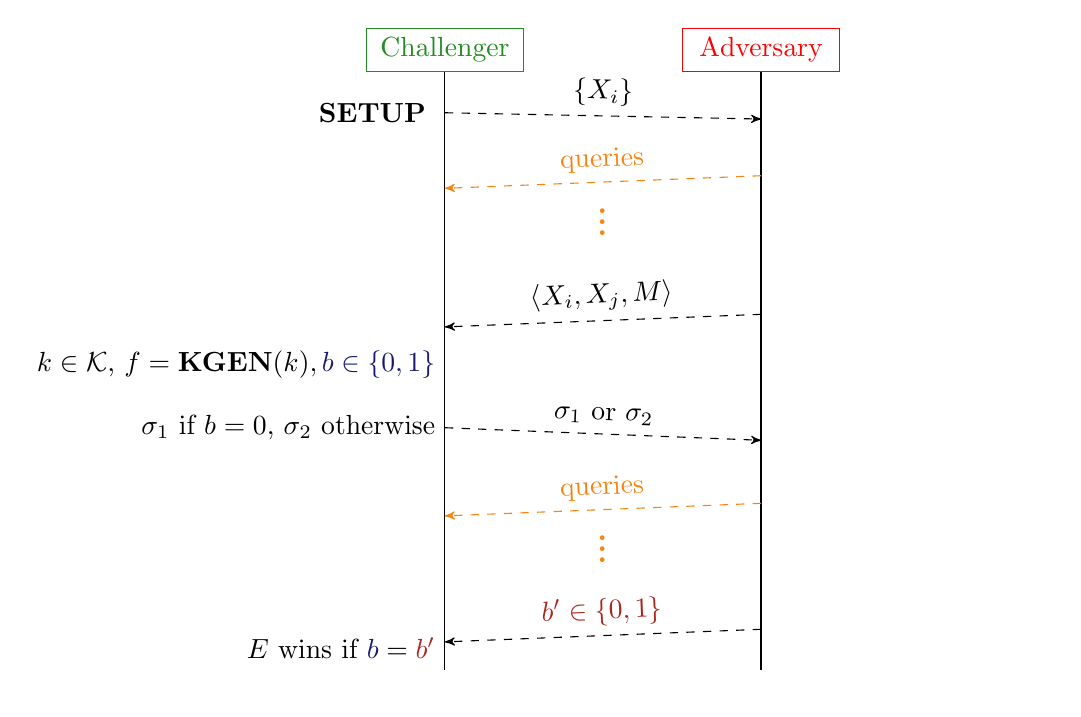
\begin{tikzpicture}[node distance=2cm,auto,>=stealth']
        \node[draw, minimum width = 2cm, color=Red] (adversary) {Adversary};
        \node[draw, minimum width = 2cm, color=ForestGreen, left = of adversary] (challenger) {Challenger};
        \node[below of=adversary, node distance=8cm] (adversaryground) {};
        \node[below of=challenger, node distance=8cm] (challengerground) {};
        
        % vertical lines
        \draw (challenger) -- (challengerground);
        \draw (adversary) -- (adversaryground);
      
        % setup
        \node[left, align=left] at ($(challenger)!0.1!(challengerground)$) {\setup};
        \visible<2->{\draw[->, dashed] ($(challenger)!0.1!(challengerground)$) -- node[sloped, above]{$\{X_i\}$} ($(adversary)!0.11!(adversaryground)$);}
        
        \visible<3->{\draw[->, dashed, BurntOrange] ($(adversary)!0.2!(adversaryground)$) -- node[sloped, above] (queries0) {queries} ($(challenger)!0.22!(challengerground)$);}
        \visible<3->{\node[below = 0mm of queries0, black] {\huge \textcolor{BurntOrange}{$\vdots$}};}

        \visible<4->{\draw[->, dashed] ($(adversary)!0.42!(adversaryground)$) -- node[sloped, above]{$\goedel{X_i, X_j, M}$} ($(challenger)!0.44!(challengerground)$);}

        \visible<5->{\node[left, align=left] at ($(challenger)!0.5!(challengerground)$) {$k\in\kspace$, $f = \textbf{KGEN}(k), \textcolor{MidnightBlue}{b\in\{0,1\}}$};}
        \visible<6->{\node[left, align=left] at ($(challenger)!0.6!(challengerground)$) {$\sigma_1$ if $b=0$, $\sigma_2$ otherwise};}

        \visible<7->{\draw[->, dashed] ($(challenger)!0.6!(challengerground)$) -- node[sloped, above]{$\sigma_1$ or $\sigma_2$} ($(adversary)!0.62!(adversaryground)$);}

        \visible<8->{\draw[->, dashed, BurntOrange] ($(adversary)!0.72!(adversaryground)$) -- node[sloped, above] (queries1) {queries} ($(challenger)!0.74!(challengerground)$);}
        \visible<8->{\node[below = 0mm of queries1, black] {\huge \textcolor{BurntOrange}{$\vdots$}};}

        \visible<9->{\draw[->, dashed] ($(adversary)!0.92!(adversaryground)$) -- node[sloped, above]{\textcolor{Mahogany}{$b'\in\{0,1\}$}} ($(challenger)!0.94!(challengerground)$);}
        
        \visible<10->{\node[left, align=left] at ($(challenger)!0.95!(challengerground)$) {$E$ wins if $\textcolor{MidnightBlue}{b}=\textcolor{Mahogany}{b'}$};}

        \node[right, align=center] at ($(adversary)!0.42!(adversaryground)$) {\phantom{{$k\in\kspace$, $f = \textbf{KGEN}(k)$}}};
      \end{tikzpicture}
    }
	\end{center}
\end{frame}

\subsection{Fairness}
\begin{frame}
	\frametitle{Fairness}

	\begin{itemize}
		\item \textbf{SETUP}, \textbf{KGen}, \textbf{KReveal}, \textbf{ASign} and \textbf{Private Key Extraction} Queries as in Ambiguity
		\item adversary $E$ outputs $S=\goedel{\underbrace{\goedel{s, h_1, f}}_{\eqqcolon\sigma},X_c, X_d, M}$
		\item Further $\averify(S)=accept$
		\item $E$ wins if one of the following holds
			\begin{itemize}
				\item $f$ was previous output from \keygen, no \textbf{KReveal} query was made and $\goedel{k, S}$ is accepted by \verify
				\item $E$ outputs $\goedel{\sigma',X_d, X_c, M'}$ with $\sigma' = \goedel{s', h_1', f}$ 
					\begin{itemize}
						\item $\averify(S') = accept$
						\item $\verify(\goedel{k,S}) = accept$
						\item $\verify(\goedel{k,S'}) = reject$
					\end{itemize}
			\end{itemize}
	\end{itemize}
\end{frame}

% --------------------------------------------------------- Proof of Lemmata
\section{Proofs}
\begin{frame}
	\frametitle{Proofs}

	\begin{itemize}
		\item Proving a lemma/theorem in depth
		\item present sketches of the remaining proofs
		\item present important bits on the secondary beamer
	\end{itemize}
\end{frame}

% --------------------------------------------------------- Conclusion
\section{Conclusion}
\begin{frame}
	\frametitle{Conclusion}

  \begin{center}  
    \begin{itemize}
      \setlength\itemsep{1em}
      \item sign entities without a significant disadvantage
      \item ambiguous until all parties are committed
      \item still not \textcolor{Plum}{\textit{truly fair}}
    \end{itemize}
  \end{center}
\end{frame}

\end{document}